\section{Distributed Database (DART)}\label{sec:DART}

\abbrev{DART}{Distributed Archive of Random Transactions}
 is built to store and keep track of transactions in the Tagion network. The database efficiently handles the removal and addition of transactions in a secure and distributed manner.
Each transaction is stored in a distributed hash-table using a cryptographic hash of the transaction T data. Each transaction is identified by a unique hash value h. The transaction is put into a table ordered by the numerical value of the hash.
\begin{equation}
 h = H(T), ~ h \in [0:2^{N-1}-1], ~ N \in \mathbb{N}
\end{equation}

\begin{equation}
  S_i \in [i \cdot 2^{N-M}:(i+1) \cdot 2^{N-M}], ~ i \in [0:m-1], ~ m = 2^M
\end{equation}


\begin{itemize}
 \item[$H$] is the cryptography hash function
 \item[$N$] represents the number of bits
 \item[$M$] represents the bit witdh of the sector
 \item[$h$]  hash value
 \item[$S$]  is sections
 \item[$m$]  hash-table divided into sections $S$
\end{itemize}

\begin{figure}[H]
 \centering
 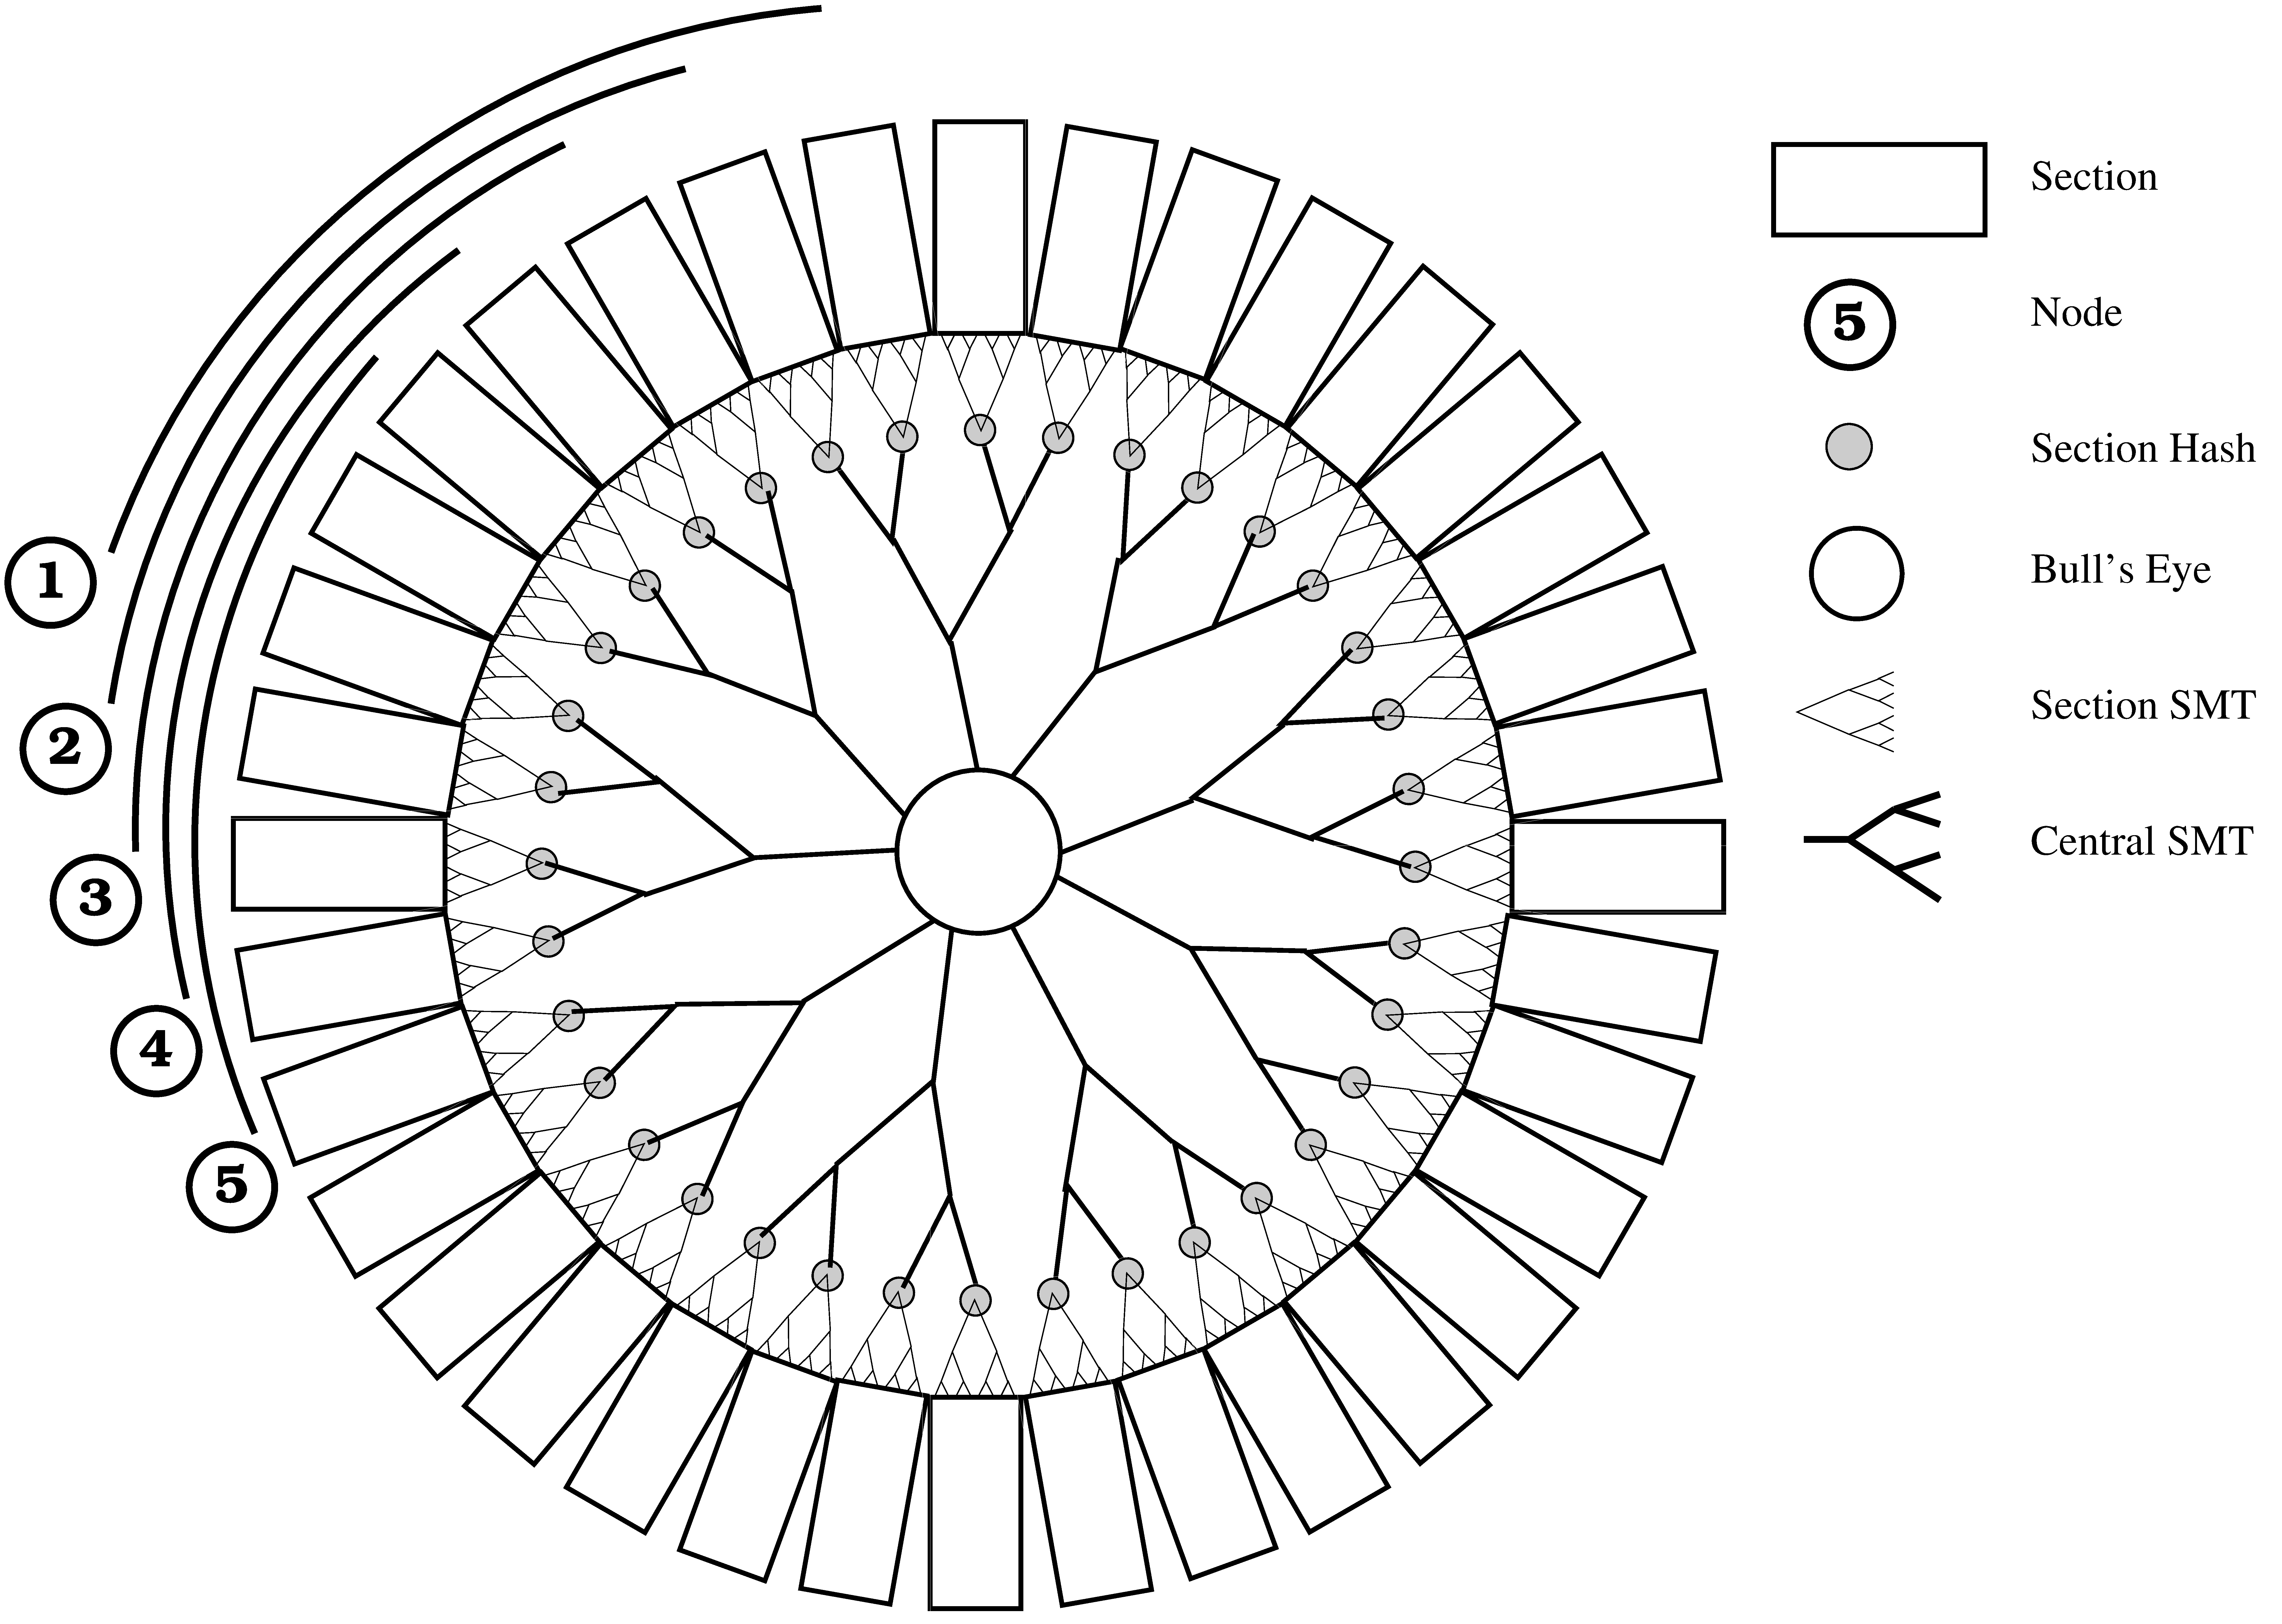
\includegraphics[width=1.0\textwidth]{fig/dart_bw.eps}
 % dart_bw.eps: 17766x12625 px, 300dpi, 150.42x106.89 cm, bb=0 0 4264 3030
 \caption{The structure of the DART database}
 \label{fig:dart}
\end{figure}


The hash-table is distributed between the nodes in the network, where each node manages a sample of sections. A section must be managed by more than Q nodes to keep redundancy and security of the data.
Each node must maintain the database sections within the node's section angle. This means adding and removing the transaction and updating the Merkle-tree root of the section hash.
The DART is updated according to the transaction list in an epoch generated by the network. The scripting engine will evaluate actions in the epoch and decide if an archive should be added, removed or selected. The selection of an archive means that the archive is sent back to the network and deleted from the DART. When a node updates a section, it must calculate the Section Merkle-root and sign it and send it to the network.
The signed section and the selected archive are distributed to the network via the gossip protocol. Each node will collect all the signed roots of the updated section when the majority has been reached for all updated sections. The node must calculate the Bull's eye (Merkle root) of the DART and sign and distribute the information via the gossip protocol. When the majority of the nodes in the network has reached a consensus of the Bull's eye value, the DART is considered to be updated.
If no consensus has been reached for DART, the current transaction in the epoch must be dropped, and the DART must revert to the previous state.
The Bull's eye value is stored in a hash-linked chain of blocks where each block points to the previous block's hash. Each block contains the Bull's eye pointer and a block number. It ensures data integrity, the state of the database. The concept is shown in the figure below.

\begin{figure}[H]
 \centering
 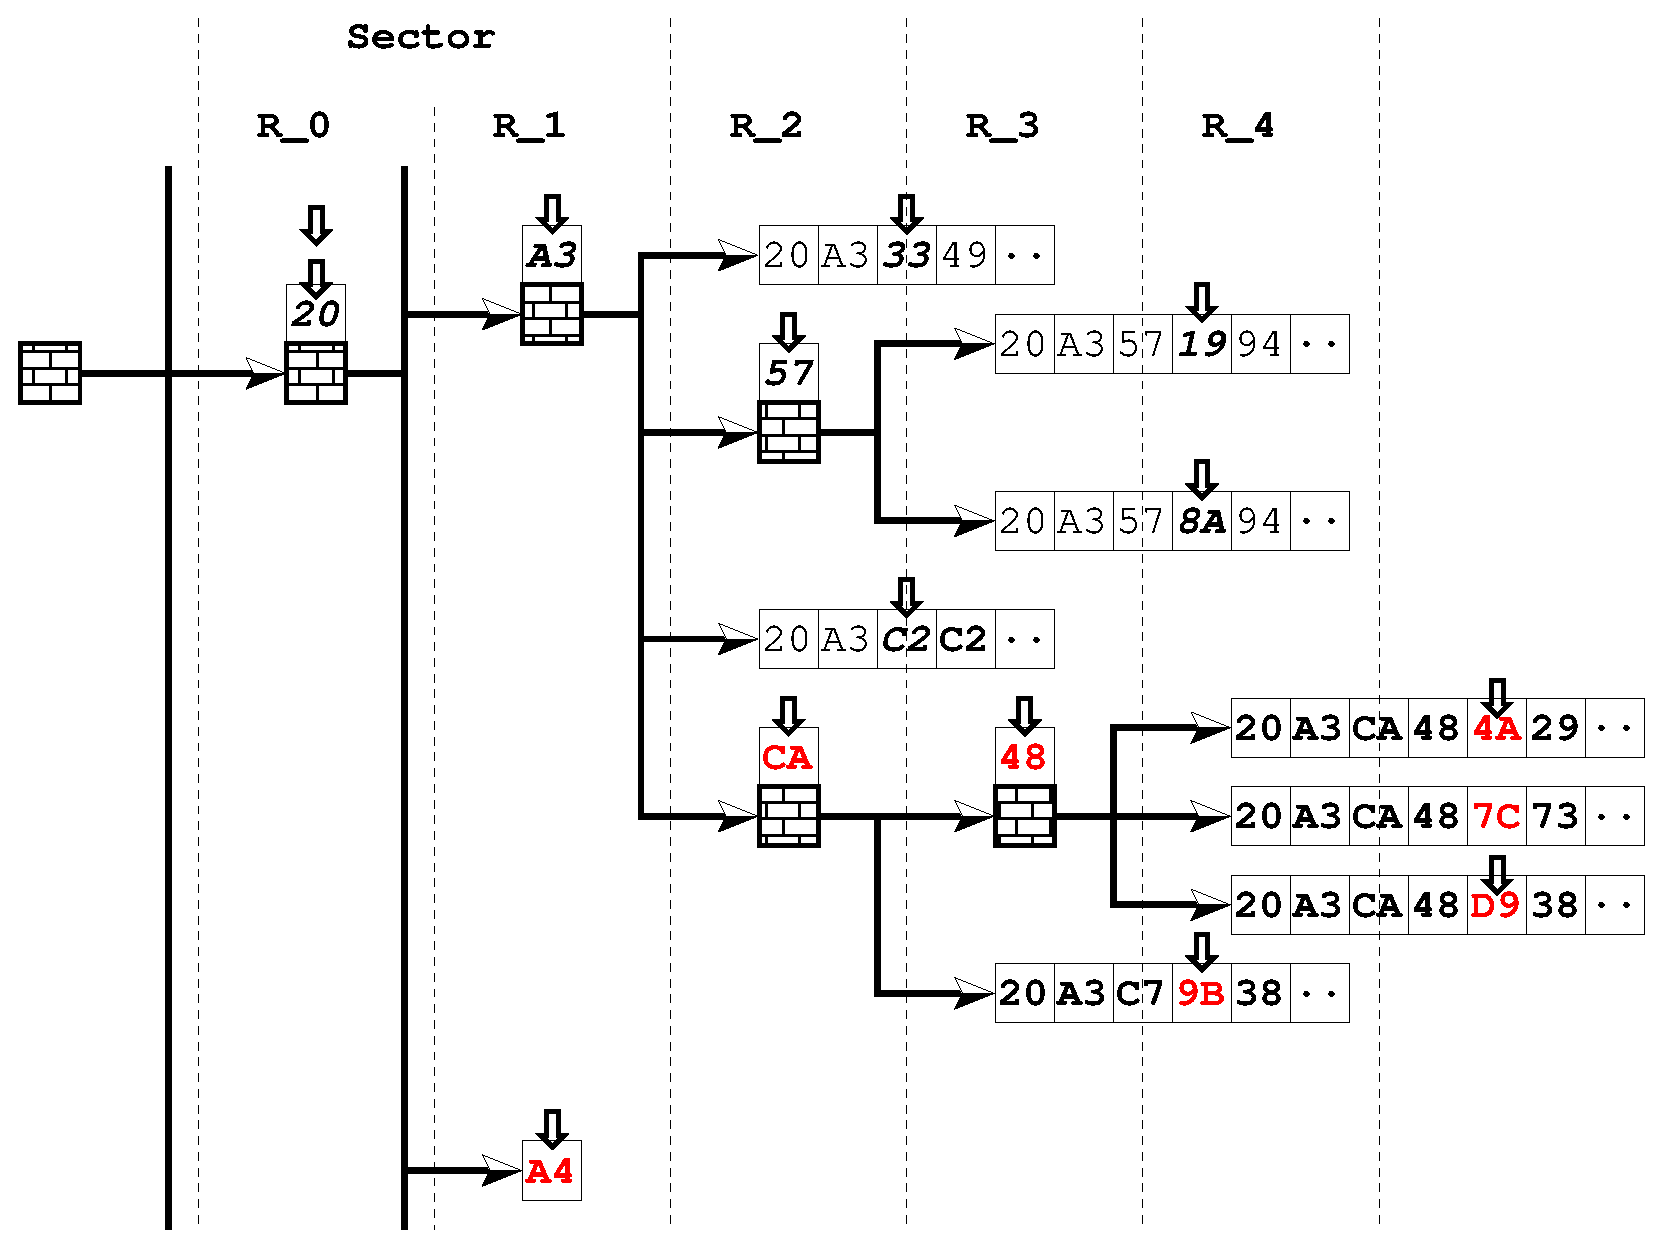
\includegraphics[width=1.0\textwidth]{fig/dart_tree_bw.eps}
 % dart_bw.eps: 17766x12625 px, 300dpi, 150.42x106.89 cm, bb=0 0 4264 3030
 \caption{The data structural layout of DART database}
 \label{fig:dart}
\end{figure}



\subsection{Sparse Merkle Tree}
The data in a section is mapped using a \abbrev{SMT}{Sparse Merkle Tree} which makes it efficient to add into and remove archives from the Merkle tree. \\
The hash point into the DART is divided by rims. Rim zero is the most significant byte (MSB) of the hash fingerprint of the archive. Rim one is the next byte in the hash etc. \\
In the current implementation of the DART, the first two rims are used as the section index. Thus the DART has a total number of indices $2^{16} = 65536$ which is equivalent to the two bytes unsigned number. \\
Each section stores the archive in a hash table. An SMT is used as a look-up table, and each rim is sectioned into a sub sparse Merkle tree. This means that rim two is the first SMT and rim three is the second SMT etc. \\ 
As a comparison, a traditional Merkle tree with $2^{24} = 8^3 \approx 16 \cdot 10^{6}$ Archives. Calculating a full Merkle tree requires the calculation of around $32 \cdot 10^6$ hashes. By contrast, using an SMT with $16 \cdot 10^{6}$  archives mean just around 2000 hashes have to be calculated.

\paragraph{Core protocol updates\\} 
The DART will be used for protocol updates by the following consensus. One or more nodes will need to run the new protocol update in a parallel DART containing the same transaction information as the current accepted DART. The new DART will have a new Bull's eye, and this will result in a fork of the Bull's eye chain. When the majority of the nodes run the newly upgraded nodes, they can decide to drop support for the old DART and run the new DART. When enough nodes stop running the old DART, it will not be able to reach a consensus, and the upgrade has completed.

\paragraph{DART garbage collection\\} 
A garbage collection script will run every (G) epoch and remove all the bills which are older than a specified date. Bills that have not been used for a long period will be burned, which ensures that the system does not contain dead bills/money.
It is the owner's responsibility to recycle their bills before the expiry date.
